
%%%%%%%%%%%%%%%%%  METHODSOVERVIEW %%%%%%%%%%%%%%%%%%%%%%%%%%%%%%%%
Throughout this paper, we use $\sL$ to denote the class of finite lattices that
are isomorphic to congruence lattices of finite algebras. 
We call the lattices that belong to $\sL$ \emph{representable} lattices. 

\section{Closure properties of the class of representable lattices}
\label{sec:clos-prop-class}
This section describes some
\emph{closure properties}
of the class $\sL$. % of representable lattices. 
By closure properties, we mean the following: if $\sansO$ is an operation that can
be applied to a lattice or collection of lattices, we say that $\sL$ is
\emph{closed under $\sansO$} provided $\sansO(\sK) \subseteq \sL$ for all 
$\sK\subseteq \sL$. For example, if 
$\sansS(\sK) = \{\text{all sublattices of lattices in $\sK$}\}$, 
it is unknown whether $\sL$ is closed under $\sansS$.  
If this were known to be true, then the 
\emph{finite lattice representation problem} would be solved.
The congruence lattice of the algebra consisting of a
set $X$ with no operations is the lattice of all equivalence relations on $X$,
which we denote by $\Eq X$.
By a celebrated theorem of \Pudlak and \Tuma~\cite{Pudlak:1980}, for every finite
lattice $L$ there is a finite set $X$ such that $L\leq \Eq X$.  Therefore, $\sL$
would contain all finite lattices if it were closed under $\sansS$.


The following is a list of operations under which $\sL$ is known to be closed,
along with the names of those who first (or independently) proved them.  We
discuss some of these results in greater detail later in this section.
The class $\sL$ of lattices isomorphic to congruence lattices of finite
algebras is closed under 
\begin{enumerate} %[label=$\circ$]
\item lattice duals\footnote{Recall, the \defn{dual of a lattice} is simply the
  lattice turned on its head, that is, the lattice obtained by
  reversing the partial order of the original lattice.}  (Hans
  Kurzweil~\cite{Kurzweil:1985} and Raimund Netter~\cite{Netter:1986}, 1986),
\item interval sublattices (follows from Kurzweil-Netter),
\item  direct products (\Jiri \Tuma~\cite{Tuma:1986}, 1986), 
\item  ordinal sums 
  (Ralph McKenzie~\cite{McKenzie:1984}, 1984; John Snow~\cite{Snow:2000}, 2000),
\item  parallel sums (John Snow~\cite{Snow:2000}, 2000), 
\item certain sublattices of lattices in $\sL$ -- namely, those which
  are obtained as a union of a filter and an ideal of a lattice in
  $\sL$ (John Snow~\cite{Snow:2000}, 2000). 
\end{enumerate}
\begin{center}
  \begin{figure}[h!]
    \label{fig:ordinal-and-parallel}
    \centering
    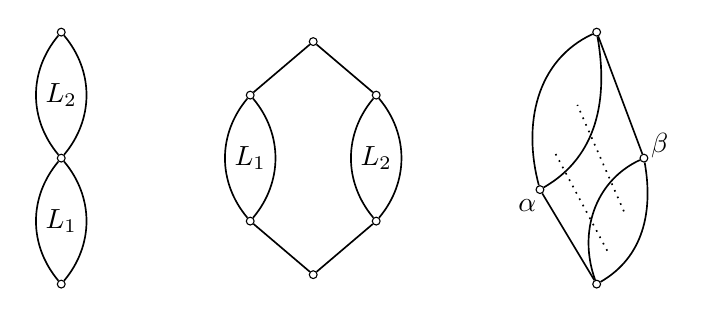
\begin{tikzpicture}[scale=0.4]

      %%% first (unlabelled) parachute %%%
      \node (botL1) at (-8,-4) [draw, circle,inner sep=1pt] {};
      \node (m80) at (-8,0) [draw, circle,inner sep=1pt] {};
      \node (topL2) at (-8,4) [draw,circle,inner sep=1pt] {};
      \node (bot) at (0,-3.7) [draw, circle,inner sep=1pt] {};
      \node (top) at (0,3.7) [draw,circle,inner sep=1pt] {};
      \node (botL) at (-2,-2) [draw,circle,inner sep=1pt] {};
      \node (topL) at (-2,2) [draw,circle,inner sep=1pt] {};
      \node (botN) at (2,-2) [draw,circle,inner sep=1pt] {};
      \node (topN) at (2,2) [draw,circle,inner sep=1pt] {};

      \draw (-8,-2) node {$L_1$};
      \draw (-8,2) node {$L_2$};
      \draw (-2,0) node {$L_1$};
      \draw (2,0) node {$L_2$};

      \draw[semithick] 
      (bot) to (botL)
      (bot) to (botN)
      (top) to (topL)
      (top) to (topN);

      \draw [semithick]  
      (botL) to [out=50,in=-50] (topL)
      (botL) to [out=130,in=-130] (topL)
      (botN) to [out=50,in=-50] (topN)
      (botN) to [out=130,in=-130] (topN);

      \draw [semithick]  
      (botL1) to [out=50,in=-50] (m80)
      (botL1) to [out=130,in=-130] (m80)
      (m80) to [out=50,in=-50] (topL2)
      (m80) to [out=130,in=-130] (topL2);

      % lat5
      \node (c) at (9.5,-3.25)   {};
      \node (d) at (7.5,0.5)   {};
      \node (e) at (10,-2)   {};
      \node (f) at (8.25,2)   {};
      \node (bottom) at (9,-4)  [draw, circle, inner sep=1pt] {};
      \node (topfi) at (9,4)  [draw, circle, inner sep=1pt] {};
      \node (alpha) at (7.2,-1)  [draw, circle, inner sep=1pt] {};
      \node (beta) at (10.5,0)  [draw, circle, inner sep=1pt] {};
      \draw[semithick, dotted] (c) to (d) (e) to (f);
      \draw[semithick] (bottom) to (alpha)  (beta) to (topfi);
      \draw[semithick] 
      (alpha) to [out=30, in=-80] (topfi)
      (topfi) to [out=205, in=105] (alpha)
      (bottom) to [out=30, in=-80] (beta)
      (beta) to [out=205, in=110] (bottom);
      \draw (6.8,-1.5) node {$\alpha$};
      \draw (11,0.4) node {$\beta$};

    \end{tikzpicture}
    \caption{The ordinal (left) and parallel (middle) sum of the lattices
      $L_1$ and $L_2$; a sublattice obtained as a union of a filter $\alpha^\uparrow $ and an ideal
      $\beta^\downarrow$ (right).}
  \end{figure}
\end{center}

\begin{remarks}
  %%   ~
  %% \begin{enumerate} %[label=$\circ$]
  %% \item  The first result says that if $L$ is representable then so is the
  The first item in the list above says that if $L$ is representable then so is the dual of $L$. 
  It follows from this that any interval sublattice of a representable lattice is
  representable.  For, let $[\alpha, \beta] := \{\theta \in L \mid \alpha \leq
  \theta \leq \beta\}$ be an interval in the representable lattice $L= \Con\bA$.
  Then $[\alpha, 1_A] \cong \Con \bA/\alpha$. By 1, the dual of $\ell := [\alpha, 1_A]$ is
  representable. %say, $\ell' = \Con \bB$. 
  Now take the filter above $\beta'$ in $\ell'$ (where $\beta'$ is the
  image of $\beta$ under dualization) and we obtain a representation of a
  lattice isomorphic to the dual of $[\alpha, \beta]$.  Apply 1
  again and we have the desired representation of $[\alpha, \beta]$.  Thus
  2 follows from 1.
  By the ordinal sum of two lattices $L_1, L_2$, we mean the lattice
  on the left of Figure~\ref{fig:ordinal-and-parallel}.
  By the parallel sum of two lattices $L_1, L_2$, we mean the lattice
  in the middle of Figure~\ref{fig:ordinal-and-parallel}.
  %% \item[4.-5.] By the
  %%   ordinal (parallel) sum of two lattices $L_1, L_2$, we mean the lattice
  %%   on the left (middle) of Figure~\ref{fig:ordinal-and-parallel}.
  Item 6 above is a very useful result which we will discuss it further in
  Section~\ref{sec:union-filter-ideal} below, where we present a short proof of
  this result. 
  Whether the class $\sL$ is closed under homomorphic images
  seems to be an open question. 
\end{remarks}

%%%%%%%%%%%%%%%%%%  METHODSINDETAIL  %%%%%%%%%%%%%%%%%%%%%%%
\subsection{Lattice duals: the theorem of Kurzweil and Netter}
\label{sec:duals-interv-subl-detail}
As mentioned above, 
the class $\sL$ -- the lattices isomorphic to congruence lattices of finite
algebras -- is closed under
dualization.
That is, if $L$ is representable, then so is the dual of $L$. This was proved in
1986 by Raimund Netter~\cite{Netter:1986}, generalizing the idea of his advisor,
Hans Kurzweil~\cite{Kurzweil:1985}. 
Though Kurzweil's article did appear (in German), it is unclear whether Netter's
article was ever published.
In this section we present a proof of their result.
The argument requires a fair bit of machinery, but it is a nice idea and
well worth the effort.\footnote{We learned 
  of the main argument used in the proof from slides of a series of three
  lectures given by P{\'e}ter \Palfy in 2009~\cite{Palfy:2009}.
  \Palfy gives credit for the argument to Kurzweil and Netter.} 

If $G$ is a group and $X$ a set, then the set $\{f \mid X\rightarrow G\}$ of 
functions from $X$ into $G$ is denoted by $G^X$.  This is a group with binary
operation $(f,g) \mapsto f\cdot g$, where,  
for each $x\in X$, $(f\cdot g)(x)= f(x)g(x)$ is simply multiplication
in the group $G$.  The identity of the group $G^X$ is of course the constant map $f(x) =
1_G$ for all $x\in X$.

Let $X$ be a finite totally ordered set, with order relation $\leq$,
and consider the set $X^X$ of functions mapping $X$ into itself.  
The subset of $X^X$ consisting of functions that are both idempotent and
decreasing\footnote{When we say that the map $f$ is ``decreasing'' we mean
  $f(x)\leq x$ for all $x$. (We do not mean $x\leq y$ implies $f(y) \leq f(x)$.)}
will be denoted by $\ID{X}$.  That is,
\[
\ID{X} = \{f\in X^X \mid f^2 = f \text{ and }\; \forall x\; f(x) \leq x\}.
\]
Define a partial order $\sqsubseteq$ on the set $\ID{X}$ by
\begin{equation}
  \label{eq:MID111}
  f\sqsubseteq g \quad \Leftrightarrow \quad \ker f \leq \ker g,
\end{equation}
where $\ker f = \{(x,y) \mid f(x) = f(y)\}$.
It is easy to see that $f\sqsubseteq g$ holds if and only if $gf = g$.  
Moreover, under this partial ordering $\ID{X}$ is a lattice which is 
isomorphic to $\bEqX$ (viz.~the map $\Theta : \EqX \rightarrow
\ID{X}$ given by $\Theta(\alpha) = f_\alpha$, where
$f_\alpha(x) = \min\{y\in X \mid (x,y)\in \alpha\}$.) % = \min x/\alpha.


Suppose $S$ is a finite nonabelian simple
group, and consider $S^n$, the direct power of $n$ copies of $S$.
An element of $S^n$ may be viewed as a map from the set 
$n = \{0, 1, \dots, n-1\}$ into $S$.  Thus, if 
$x = (x_0, x_1, \dots, x_{n-1})\in S^n$, then by 
$\ker x$ we mean the relation $(i,j) \in \ker x$ if and only if $x_i = x_j$.
The set of constant maps is a subgroup $D < S^n$, sometimes called the
\defn{diagonal subgroup}; that is,
$D = \{(s, s, \dots, s) \mid s\in S\} \leq S^n$.

For each $f \in \ID{n}$, define
\[
K_f = \{(x_{f(0)}, x_{f(1)}, \dots, x_{f(n-1)}) \mid x_{f(i)}\in S, \; i = 0, 1,
\dots, n-1\}.
\]
Then $D \leq K_f\leq S^n$, and $K_f$ is the set of maps
$K_f = \{x f \in S^n \mid x \in S^n \}$; i.e., compositions of the given
map $f\in n^n$, followed by  any $x\in S^n$.  Thus, 
$K_f = \{ y\in S^n \mid \ker f \leq \ker y \}$.
For example, 
if $f = (0, 0, 2, 3, 2)\in \ID{5}$, then 
$\ker f = |0,1|2,4|3|$ and 
$K_f$ is the subgroup %$\Delta \leq K_f \leq S^5$ 
of all $(y_0, y_1, \dots, y_4)\in S^5$ having $y_0 = y_1$ and $y_2 = y_4$. That is,
$K_f = \{(x_{0}, x_{0}, x_2, x_3, x_2) \mid x\in S^5\}$.

\begin{lemma}
  \label{lem:latt-duals}
  The map $f \mapsto K_f$ is a dual lattice isomorphism from $\bEq(n)$ onto the
  interval sublattice $[D, S^n] \leq \Sub(S^n)$.
\end{lemma}
\begin{proof}
  This is clear since $\ID{n}$ is ordered by (\ref{eq:MID111}), and 
  we have 
  $f\sqsubseteq h$ if and only if
  $K_h = \{y \in S^n \mid \ker h \leq \ker y \}
  \leq \{y \in S^n \mid \ker f \leq \ker y \} =  K_f$.
\end{proof}

\begin{theorem}[Kurzweil~\cite{Kurzweil:1985}, Netter~\cite{Netter:1986}]
  \label{thm:duals-interv-subl}
  If the finite lattice $L$ is representable (as the congruence lattice of a
  finite algebra), then so is the dual lattice $L'$.
\end{theorem}
\begin{proof}
  Without loss of generality, we assume that $L$ is represented
  as $L = \Con \<n, F\>$.
  Also, by \cite[Theorem~4.18]{alvi:1987}, we can assume
  that $F$ consists of unary operations: $F \subseteq n^n$.  
  As above, let $S$ be a nonabelian simple group
  and let $D$ be the diagonal subgroup of $S^n$.
  Then the unary algebra $\<S^n/D, S^n\>$  is a transitive $S^n$-set which (by
  Theorem~\ref{thm:g-set-isomorphism2} below) has congruence lattice isomorphic
  to the interval $[D, S^n]$.  By Lemma~\ref{lem:latt-duals}, this is the dual
  of the lattice $\bEq(n)$.  That is, 
  $\Con \<S^n/D, S^n\> \cong (\bEq(n))'$.

  \todo{Replace the reference to Theorem~\ref{thm:g-set-isomorphism2} with a
    reference to the appropriate theorem in ALVIN, since the section containing
    Theorem~\ref{thm:g-set-isomorphism2} below will be deleted.}

  
  Now, each operation $\phi \in F$ gives rise to an operation on $S^n$
  by composition:
  \[
  \hat{\phi}(\bs) = \hat{\phi}(s_{0}, s_1  \dots, s_{n-1}) = (s_{\phi(0)},
  s_{\phi(1)}\dots, s_{\phi(n-1)}). 
  \]
  Thus, $\phi$ induces  an operation on $S^n/D$ since, for 
  $\bd = (d, d, \dots, d) \in D$ and $\bs \in S^n$ we have 
  $\bs \bd = (s_{0}d, s_{1}d, \dots , s_{n-1}d)$ and 
  $\hat{\phi}(\bs \bd) = (s_{\phi(0)}d, s_{\phi(1)}d, \dots , s_{\phi(n-1)}d) = \hat{\phi}(\bs) \bd$,
  so $\hat{\phi}(\bs D)  = \hat{\phi}(\bs) D$.  Finally, add the set of operations 
  $\hat{F} = \{\hat{\phi} \mid \phi \in F\}$ to $\<S^n/D, S^n\>$, yielding the
  new algebra  $\<S^n/D, S^n \cup \hat{F}\>$, and observe
  that a congruence $\theta \in \Con\<S^n/D, S^n\>$ remains a congruence of
  $\<S^n/D, S^n \cup \hat{F}\>$ if and only if it correponds to a partition on
  $n$ that is invariant under $F$.
\end{proof}

\todo{Perhaps we should give more details in the last sentence of the proof.}
%   Some notes are below, but they need to be cleaned up.}

%% {\it Notes on the last sentence of the proof:}
%% Fix 
%% $\theta \in \Con \< S^{n}/D, S^{n}\> \cong [D, S^n]$.  Then\footnote{This,
%%   and more generally the isomorphism $\Con \< S^{n}/D, S^{n}\> \cong [D, S^n]$
%%   follows from Theorem~\ref{thm:g-set-isomorphism2} below.} there corresponds a
%% subgroup $D \leq K_f \leq S^n$ such that 
%% $(x,y)\in \theta$ iff $x^{-1}y = z\in K_f$.  Now if $\hat{\phi}\in \hat{F}$, then
%% $(\hat{\phi}x, \hat{\phi}y) \in \theta$ iff 
%% \[
%% (x_{\phi(0)}^{-1}y_{\phi(0)}, \dots,  x_{\phi(n-1)}^{-1} y_{\phi(n-1)}) =
%% (z_{\phi(0)},z_{\phi(1)},\dots, z_{\phi(n-1)})\in K_f.
%% \]
%% Better: Take $z\in K_f$ with $\ker z = \ker f$, so $f(i)=f(j)$ iff $z_i = z_j$.
%% Now suppose $\phi\in F$ does not respect $\ker f$, so there exists $(i,j) \in
%% \ker f$ such that $(\phi(i), \phi(j)) \notin \ker f$.  Then $\phi z \notin K_f$,
%% since $z_{\phi(i)} \neq z_{\phi(j)}$.

\subsection{Union of a filter and ideal}
\label{sec:union-filter-ideal}
The lemma in this section was originally proved by John Snow using primitive positive
formulas.  Since it provides such a useful tool for proving that certain finite lattices 
are representable as congruence lattices, we give our own direct
proof of the result below. 

Before stating the lemma, we need a couple of definitions.  (These will be
discussed in greater detail in Section~\ref{sec:closure-method}.)
Given a relation $\theta \subseteq X\times X$, we say that the map 
$f: X^n\rightarrow X$ \emph{respects} $\theta$ and we write 
$f(\theta) \subseteq \theta$ provided $(x_i, y_i)\in \theta$ implies
$(f(x_1, \dots, x_n), f(y_1, \dots, y_n))\in \theta$.
For a set $L\subseteq \Eq X$ of equivalence relations we define
\[
\lambda(L) = \{f\in X^X: (\forall \theta \in L) \; f(\theta) \subseteq \theta \},
\]
which is the set of all unary maps on $X$ which respect all relations in $L$.
\begin{lemma} 
  \label{lemma:union-filter-ideal}
  Let $X$ be a finite set.
  If $\bL \leq \bEqX$ is representable and $\bL_0\leq \bL$ is a sublattice with universe
  $\upalpha\cup \downbeta$ where $\upalpha=\{x\in L \mid \alpha \leq x\}$ and 
  $\downbeta=\{x\in L \mid x\leq \beta\}$ for some $\alpha, \beta \in L$, then $\bL_0$ is representable.
\end{lemma}

\vskip3mm

\begin{center}
  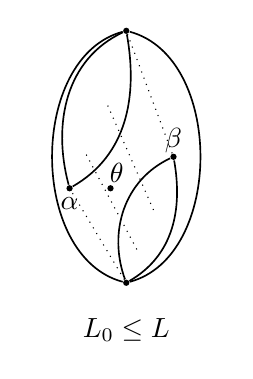
\begin{tikzpicture}[scale=.4]
    % lat5
    \node (c) at (.5,.75)   {};
    \node (d) at (-1.5,4.5)   {};
    \node (e) at (1,2)   {};
    \node (f) at (-.75,6)   {};
    \node (bottom) at (0,0)  [fill, circle, inner sep=.8pt] {};
    \node (top) at (0,8)  [fill, circle, inner sep=.8pt] {};
    \node (alpha) at (-1.8,3)  [fill, circle, inner sep=.8pt] {};
    \node (beta) at (1.5,4)  [fill, circle, inner sep=.8pt] {};
    \node (theta) at (-.5,3)  [fill, circle, inner sep=.8pt] {};
    \draw (-.3,3.5) node {$\theta$};
    \draw[semithick] 
    (bottom) to [out=15, in=-15] (top) 
    (top) to [out=195, in=165] (bottom);
    \draw[dotted] (c) to (d) (e) to (f);
    \draw[dotted] (bottom) to (alpha)  (beta) to (top);
    \draw[semithick] 
    (alpha) to [out=30, in=-80] (top)
    (top) to [out=205, in=105] (alpha)
    (bottom) to [out=30, in=-80] (beta)
    (beta) to [out=205, in=110] (bottom);
    \draw (0,-1.5) node {$L_0 \leq  L$};
    \draw (-1.8,2.5) node {$\alpha$};
    \draw (1.5,4.5) node {$\beta$};
  \end{tikzpicture}
\end{center}

\vskip3mm

\begin{proof}
  Assume $\bL_0 \ncong \two$, otherwise the result holds trivially. 
  Since $\bL\leq \bEqX$ is representable, we have $\bL = \bCon
  \<X, \lambda(L)\>$ (cf.~Section~\ref{sec:closure-method}).  Take an arbitrary
  $\theta \in L \setminus L_0$. Since $\theta \notin \upalpha$, 
  % -- that is, $\alpha$ is not below $\theta$ --  
  there is a pair 
  $(a,b) \in \alpha \setminus \theta$.  Since $\theta \notin \downbeta$, there is
  a pair $(u,v)\in \theta\setminus \beta$. Define $h\in X^X$ as follows:
  \begin{equation*}
    h(x) = \begin{cases}
      a,& \quad x\in u/\beta,\\
      b,& \quad \text{ otherwise.}
    \end{cases}
  \end{equation*}
  Then, $\beta \leq \ker h = (u/\beta)^2 \cup ((u/\beta)^c)^2$, where $(u/\beta)^c$ denotes the
  complement of the $\beta$ class containing $u$.  Therefore, $h$ respects every
  $\gamma \leq \beta$.  Furthermore, $(a, b) \in \gamma$ for all $\gamma \geq \alpha$,
  so $h$ respects every $\gamma$ above $\alpha$.  This proves that $h\in \lambda(L_0)$.
  Now, $\theta$ was arbitrary, so we have proved that for every $\theta \in L
  \setminus L_0$ there exists a function in $\lambda(L_0)$ which respects every
  $\gamma \in \upalpha\cup \downbeta = L_0$, but violates $\theta$.  Finally,
  since 
  $\bL_0 \leq \bL$, we have $\lambda(L)\subseteq \lambda(L_0)$.  Combining these
  observations, we see that every $\theta \in \Eq X \setminus L_0$ is
  violated by some function in $\lambda(L_0)$. Therefore, $\bL_0 = \bCon \< X, \lambda(L_0)\>$.
\end{proof}

\subsection{Ordinal Sums I}
\label{sec:ordinal-sums}
\todo{Revise this section.  Peter has written up some nice lemmas and
  theorems on this topic which now appear below in a subsection called
  ``Ordinal Sums II,'' but that material should be integrated with and/or
  replace the material in this subsection.} 

The following theorem is a consequence of 
McKenzie's shift product construction~\cite{McKenzie:1984}. %, which we describebriefly below.
% \todo{Possibly add a short description of the shift product.}
\begin{theorem}
  \label{thm:ordinal-sums}
  If $L_1, \dots, L_n \in \sL$ is a collection of representable lattices, then
  the ordinal sum and the adjoined ordinal sum, shown in
  Figure~\ref{fig:adjordinal}, are representable.
\end{theorem}
A more direct proof of Theorem~\ref{thm:ordinal-sums} follows the argument given
by John Snow in~\cite{Snow:2000}.  As noted above, 
\Jiri \Tuma proved that
the class of finite representable lattices is closed under direct products.
Thus, if $L_1$ and 
$L_2$ are representable, then so is $L_1 \times L_2$.  Now note that the
adjoined ordinal sum of $L_1$ and $L_2$ is the union, $\alpha^\uparrow \cup
\beta^\downarrow$,  of a filter and ideal  
in the lattice $L_1 \times L_2$, where
$\alpha = \beta = 1_{L_1} \times 0_{L_2}$.  
Therefore, by Lemma~\ref{lemma:union-filter-ideal},
the adjoined ordinal sum is representable.  A trivial induction argument proves the
result for adjoined ordinal sums of $n$ lattices.  The same result for ordinal
sums (Figure~\ref{fig:adjordinal} left) follows since the two element lattice is
obviously representable. 

\begin{center}
  \begin{figure}[h!]
    \label{fig:adjordinal}
    \centering
        {\scalefont{.8}
          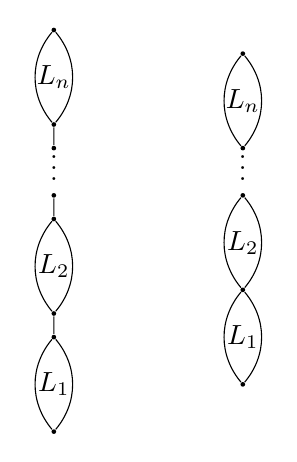
\begin{tikzpicture}[scale=0.3]
            \node (botL1) at (8,-4) [fill, circle,inner sep=.6pt] {};
            \node (00) at (8,0) [fill, circle,inner sep=.6pt] {};
            \node (topL2) at (8,4) [fill,circle,inner sep=.6pt] {};
            \node (topLn) at (8,10) [fill, circle,inner sep=.6pt] {};
            \node (botLn) at (8,6) [fill, circle,inner sep=.6pt] {};

            \draw (8,-2) node {$L_1$};
            \draw (8,8) node {$L_n$};
            \draw (8,2) node {$L_2$};
            \draw (8,5.5) node {$\vdots$};

            \draw 
            (botL1) to [out=50,in=-50] (00)
            (botL1) to [out=130,in=-130] (00)
            (00) to [out=50,in=-50] (topL2)
            (00) to [out=130,in=-130] (topL2)
            (botLn) to [out=50,in=-50] (topLn)
            (botLn) to [out=130,in=-130] (topLn);

            \node (botL1) at (0,-6) [fill, circle,inner sep=.6pt] {};
            \node (topL1) at (0,-2) [fill, circle,inner sep=.6pt] {};
            \node (botL2) at (0,-1) [fill, circle,inner sep=.6pt] {};
            \node (topL2) at (0,3) [fill,circle,inner sep=.6pt] {};
            \node (04) at (0,4) [fill, circle,inner sep=.6pt] {};
            \node (06) at (0,6) [fill, circle,inner sep=.6pt] {};
            \node (botLn) at (0,7) [fill, circle,inner sep=.6pt] {};
            \node (topLn) at (0,11) [fill, circle,inner sep=.6pt] {};

            \draw (0,-4) node {$L_1$};
            \draw (0,9) node {$L_n$};
            \draw (0,1) node {$L_2$};
            \draw (0,5.5) node {$\vdots$};

            \draw 
            (botL1) to [out=50,in=-50] (topL1)
            (botL1) to [out=130,in=-130] (topL1) 
            to (botL2) to [out=50,in=-50] (topL2)
            (botL2) to [out=130,in=-130] (topL2)
            (topL2) to (04)
            (06) to (botLn) to [out=50,in=-50] (topLn)
            (botLn) to [out=130,in=-130] (topLn);
          \end{tikzpicture}
        }
        \caption{The ordinal sum (left) and the adjoined ordinal sum (right) of the lattices
          $L_1, \dots, L_n$.}
  \end{figure}
\end{center}

\subsection{Ordinal Sums II}
\todo{Merge this subsection with the subsection ``Ordinal Sums I.''}
\newcommand{\m}{\mathbf}

The lattice of equivalence relations on an $n$-element set is denoted by
Equ$(n)$. For two lattices $\m L,\m M$ the \emph{adjoined ordinal sum}  
is denoted by $\m L\oplus_a \m M$ and is defined on $L\uplus (M\setminus\{0\})$
by $x\le y$ iff $x\in L,y\in M$ or ($x,y\in L$ and $x\le^\m L y$) or ($x,y\in M$
and $x\le^\m M y$). 

Let $\m A,\m B$ be two finite algebras of cardinality $m$ and $n$ respectively,
and let $\m L=\text{Con}(\m A)$ and $\m M=\text{Con}(\m B)$. 
In \cite{Snow:2000} it is proved that $\m L\oplus_a\m M$ is isomorphic to the
congruence lattice of some finite algebra $\m C$. Although the algebra $\m C$ is
not explicitly constructed, it is based on the direct product of $\m A$ and $\m
B$, hence the ordinal sum is a sublattice of Equ$(mn)$. Here we give a different
construction of $\m C$ that leads to a tighter representation of Con$(\m C)$ as
a sublattice of Equ$(m+n-1)$.  
%If $\m A$ and $\m B$ are minimal-size algebras that have congruence lattices
%isomorphic to $\m L$ and $\m M$ respectively, then $\m C$ will also be a
%minimal-size algebra with congruence lattice isomorphic to $\m L\oplus_a\m M$. 

Define a unary algebra $\m A_{m,n}$ with $m+n-1$ elements as follows: 
the base set is $A\uplus B_1$ where $A=\{a_0,\dots,a_{m-1}\}$,
$B_1=\{b_1,\dots,b_{n-1}\}$ and for each function $h:B_1\to A$ define a unary
operation 
$$\hat h(x)=\begin{cases}h(x)&\text{if $x\in B_1$}\\ 
x&\text{otherwise.}\end{cases}$$

\begin{lemma}
  For $m,n\ge 1$ the lattice $\mathrm{Con}(\m A_{m,n})$ is isomorphic to
  $\mathrm{Equ}(m)\oplus_a \mathrm{Equ}(n)$. 
\end{lemma}
\begin{proof}
  Let $\alpha$ be the equivalence relation
  $A^2\cup\{(b_1,b_1),\dots,(b_{n-1},b_{n-1})\}$, so as a partition it is  
  $a_0,\dots,a_{m-1}|b_1|b_2|\dots|b_{n-1}$. 
  Note that Equ$(m)\oplus_a \text{Equ}(n)$ is isomorphic to the sublattice
  of Equ$(A\uplus B_1)$ of all equivalence relations comparable to $\alpha$, since
  $\alpha$ has a unique non-singleton block of size $m$, and $n$ blocks
  altogether. We claim that this sublattice is the congruence lattice of $\m
  A_{m,n}$.  

  Suppose $\theta\le\alpha$, and let $(x,y)\in\theta$. Then $x,y\in A$ or $x=y$,
  hence for any operation $\hat h$ we  have $\hat h(x)=x$ and $\hat h(y)=y$ or
  $\hat h(x)=\hat h(y)$, so $(\hat h(x),\hat h(y))\in\theta$. 

  Suppose $\alpha\le\theta$, and let $(x,y)\in\theta$. Since $A^2\subseteq\alpha$
  and since the range of each $\hat h$ is $A$ it follows that 
  $(\hat h(x),\hat h(y))\in\theta$. 

  Now suppose $\theta$ is incomparable with $\alpha$. Then $A^2$ is not a subset
  of $\theta$, hence there exist $(x,y)\in A^2\setminus\theta$ and
  $(u,v)\in\theta\setminus\alpha$. If $u,v\in B_1$ then choose a function $h$ (as
  in the definition of $\m A_{m,n}$) such that $h(u)=x$ and $h(v)=y$, in which
  case $\hat h$ is an operation that shows $\theta$ is not a congruence. 
  If $u\in B_1$, but $v\in A$, note that we cannot have both $(x,v)$ and $(y,v)$
  in $\theta$ (else $(x,y)\in\theta$). Assume without loss of generality 
  that $(x,v)\notin\theta$ and choose $h$ such that $h(u)=x$, then again $\hat h$
  shows that $\theta$ is not a congruence. 
  The case $u\in A$, $v\in B_1$ is similar, and $u,v\in A$ is excluded since
  $(u,v)\notin\alpha$. 
\end{proof}

%\newpage

\begin{theorem}
  Suppose $\m A=(A,F)$ and $\m B=(B,G)$ are unary algebras with
  $A=\{a_0,\dots,a_{m-1}\}$, $B=\{b_0,\dots,b_{n-1}\}$ and 
  $A\cap B=\{a_0\}=\{b_0\}$ $($so $a_0,b_0$ are identified$)$. Let $\m C$ be the
  algebra $\m A_{m,n}$ expanded with the operations 
  $$
  \hat f(x)=\begin{cases}f(x)&\text{if $x\in A$}\\
  f(a_0)&\text{otherwise}\end{cases}\qquad\qquad
  \hat g(x)=\begin{cases}g(x)&\text{if $x\in B$}\\
  g(b_0)&\text{otherwise}\end{cases}
  $$
  for $f\in F$ and $g\in G$. Then $\mathrm{Con}(\m C)$ is isomorphic to
  $\mathrm{Con}(\m A)\oplus_a\mathrm{Con}(\m B)$. 
\end{theorem}

\begin{proof}
  Since $\m C$ is an expansion of $\m A_{m,n}$ it follows from the preceding lemma
  that Con$(\m C)$ is a sublattice of 
  $\{\theta\in \text{Equ}(A\cup B):\theta\le\alpha$ or $\alpha\le\theta\}$ where,
  as before, $\alpha=A^2\cup\text{id}_B$. Note that $\alpha\in\text{Con}(\m C)$,
  so it suffices to show that $\{\theta\in\text{Con}(\m C):\theta\le\alpha\}$ is
  isomorphic to Con$(\m A)$ and $\{\theta\in\text{Con}(\m C):\theta\le\alpha\}$ 
  is isomorphic to Con$(\m B)$. The second isomorphism follows from the
  observation that $\m C/\alpha$ is isomorphic to $\m B$ via the map 
  $A\mapsto b_0$ and $\{b_i\}\mapsto b_i$ for $i\ge 1$. For the first isomorphism,
  note that the operations $\hat g$, $\hat h$ preserve all equivalence relations
  below $\alpha$. Similarly it is straight forward to check that $\hat f$
  preserves $\theta\le\alpha$ iff $f$ preserves $\theta\cap A^2$. 
  Hence the map $\theta\mapsto\theta\cap A^2$ is the required isomorphism.
\end{proof}

Now assume $\m A$ and $\m B$ are minimal-size algebras with congruence lattices
isomorphic to $\m L$ and $\m M$ respectively. Then it seems likely that the
algebra $\m C$ above is minimal in size with respect to having a congruence
lattice isomorphic to $\m L\oplus_a\m M$. Suppose $\m C'$ is a smaller algebra
with the same congruence lattice, and let $\alpha$ be the congruence in the
``middle'' of the ordinal sum. Then $\m C'/\alpha$ has a congruence lattice
isomorphic to $\m M$, hence $|\m C'/\alpha|=|\m B|=$ number of blocks in
$\alpha$. However, $\alpha$ does not need to have a unique nontrivial block, so
it is not clear at the moment how to obtain a smaller algebra $\m A'$ such that
Con$(\m A')$ is isomorphic to $\m L$. 


